\documentclass{stats_apa_style2}

\usepackage{url}
\usepackage[tmargin=1in,bmargin=1in,lmargin=1.25in,rmargin=1.25in]{geometry}
\usepackage{minted}
\usepackage{graphicx}
\usepackage{subcaption}
\usepackage{apacite}
\usepackage{graphicx}
\usepackage{filecontents}
\usepackage{float}
\usepackage{caption}

\begin{filecontents*}{MyReferences.bib}
@article{marlow2000spending,
  title={Spending, school structure, and public education quality. Evidence from California},
  author={Marlow, Michael L},
  journal={Economics of Education Review},
  volume={19},
  number={1},
  pages={89--106},
  year={2000},
  publisher={Elsevier}
}
@article{dill2005academic,
  title={Academic quality, league tables, and public policy: A cross-national analysis of university ranking systems},
  author={Dill, David D and Soo, Maarja},
  journal={Higher education},
  volume={49},
  number={4},
  pages={495--533},
  year={2005},
  publisher={Springer}
}
@article{murias2008composite,
  title={A composite indicator for university quality assesment: The case of Spanish higher education system},
  author={Murias, Pilar and de Miguel, Jos{\'e} Carlos and Rodr{\'\i}guez, David},
  journal={Social Indicators Research},
  volume={89},
  number={1},
  pages={129--146},
  year={2008},
  publisher={Springer}
}
@article{van2009does,
  title={Does university quality drive international student flows?},
  author={Van Bouwel, Linda and Veugelers, Reinhilde},
  journal={Available at SSRN 1538118},
  year={2009}
}
@article{mcaleer2005ten,
  title={The Ten Commandments for ranking university quality},
  author={McAleer, Michael},
  journal={Journal of Economic Surveys},
  volume={19},
  number={4},
  pages={649--653},
  year={2005},
  publisher={Wiley Online Library}
}
@article{gonzalez2006dimensions,
  title={Dimensions for evaluating university quality in the European Space for Higher Education},
  author={Gonz{\'a}lez-L{\'o}pez, Ignacio},
  journal={Electronic journal of research in educational psychology},
  volume={4},
  number={3},
  pages={445--468},
  year={2006},
  publisher={University of Almeria, Education \& Psychology I+ D+ i. Faculty of Psychology Department of Educational and Developmental Psychology, Carretera de Sacramento s/n, 04120 LaCanada de San Urbano, Almeria, Spain}
}
@misc{timesdata,
  title={World University Rankings 2011-2016},
  author={{\relax Times Higher Education}},
  year={2016},
  url={https://www.kaggle.com/mylesoneill/world-university-rankings}
}
@misc{shanghaidata,
  title={Academic Ranking of World Universities 2011-2015},
  author={{\relax Shanghai Ranking Consultancy}},
  year={2015},
  url={https://www.kaggle.com/mylesoneill/world-university-rankings}
}
@misc{worldbank,
  title={World Development Indicators},
  author={{\relax The World Bank}},
  year={2016},
  url={http://data.worldbank.org/indicator}
}
\end{filecontents*}

\title{Building a Linear Model to Explain University Ranking}
\author{Dylan Goldsborough and Geert Konijnendijk}
\date{\today}
\course{Experimental Design and Data Analysis}
\instructor{Instructor: Eduard Belitser}
\university{University of Amsterdam}
\shorttitle{Explaining University Ranking}

\begin{document}

\maketitle

%\begin{abstract}
%\noindent
%\end{abstract}

%\newpage

\section*{Introduction}

% General introduction
With the increasing globalization of the world, it is becoming significantly
easier to study at any given university, regardless of one's country of origin.
With the creation of this opportunity to study anywhere, the practice of ranking
universities has taken off. Nowadays, many different institutions monitor the
quality of universities worldwide, and publish annual rankings. Examples of
these institutions are the Times Higher Education magazine, the Shanghai Ranking
Consultancy and the Center for World University Rankings. These scores can have
great effects on which universities are preferrably attended by students, and
can even direct the flows of international students. In a study by
\citeA{van2009does}, it was found that the Shanghai ranking has a great
explanatory power in predicting where students will choose to attend university,
as students tend to move from countries with low scores to countries with higher
scores. With the availability of data on the quality of universities, the
question can be asked what causes the quality of some universities to be higher
than the quality of others. Is the spread around the world random, or are there
traits exhibited by countries and regions that allow great universities to
emerge?
Are there economic factors that make a difference? And are there general traits of the
university that affect the quality of education? 

% What makes a good university?
University ranking in general is not an easy assessment, demonstrated by the
large number of different university rankings that disagree on the exact
ordering of all universities. It is still disputed what the right way is to rank
universities, as many rankings are heavily criticized on factors such as the
indicators of quality they chose or their statistical inaccuracy
\cite{dill2005academic}. However, according to this study, the factors chosen to
represent quality accross rankings are becoming increasingly in agreement with
each other.

In general, there are a number of factors that are looked at to assess the
quality of a school. One broad category of indicators are research achievements
related to the institution. In this category, the quality of the school is
judged by the number of academic awards won by alumni and staff, the number of
papers annually published in renowned scientific journals, and how often
researchers at this university are cited \cite{shanghaidata}. The second broad
category regards teaching quality, and regards the staff-to-student ratio, the
available funds for teaching, and the number of international students
\cite{timesdata}. Finally, some rankings attempt to supplement the resulting
score with a reputation survey, performed on an annual basis \cite{timesdata}.
There is debate on whether variables related to the service to students should
be included. An example is a score suggested by \citeA{murias2008composite},
which includes availability of study places and ability to enroll in the
students' chosen courses without oversubscription issues. Another survey also
found that students themselves found the quality of service to them the most
important factor in quality, instead of research achievements of the school
\cite{gonzalez2006dimensions}. These factors are not without scrutiny: according
to \citeA{mcaleer2005ten}, factors such as school size are often not taken into
account in the right way, as school-wide statistics are used instead of
per-student counts.

To determine a score from the different factors, two different methods are used
\cite{dill2005academic}. Some rankings, such as the Shanghai ranking, use and aggregate the raw scores, with
weights for each factor. Others use a weighted aggregate of the rankings for each
factor, and use this to determine their final ranking.

% What variables shall we look at? University specific and country specific
Only a limited amount of research has been done to answer the question what
allows high quality education to emerge. Typically, studies focus on a
smaller scale, often an area within the United States, or on high school
education.
A study by \citeA{marlow2000spending} gives us some insight in the type of model
that can be built to explain education quality. He built a linear multiple
regression model to explain quality of public education in California. Factors
he includes are the GDP per capita in the area, the population density, the
student share of the population and the education spending per student. The
variable population density is mostly interesting on a local scale, as it
carries information about the neighborhood a school is located in. As
universities draw students from all over the country this variable is not as
meaningful, so for explaining university ranking this is not interesting. The
education spending, student share of the population and GDP per capita, however,
might be of interest.

% Government expenditure per tertiary student as % of GDP per capita (%)
There are several other factors that have not been utilized in this study, but
could be interesting in the context of university quality. The interest rate on
loans could be interesting, as tuition fees are expensive in many countries, and
student loans obligatory as a result. It might also be interesting to see if an
interaction is present between income per capita and the
effect of loan interest rates, as higher income could lessen the need for loans, and thus lessen any effect that interest rate has. The percentage of the population with internet access could be an
interesting operationalization of how modern the country is, which could also
affect the quality of the universities in this country. According to
\citeA{mcaleer2005ten}, one important factor in the quality of a university
education is the size of the university. Finally, we can test if there are differences in 
the university quality based on the continent on which the university is located.

% Formulate a research question
In this study we aim to build a model to explain the quality of university
education. To produce models, we will use multiple regression, ANOVA and an ANCOVA.
We use data from the Shanghai Ranking Consultancy as dependent variable. The
country-specific explanatory variables used to construct the models are GDP per capita,
education spending per student, the loan interest rate, the percentage of the population with internet access, and
the continent on which the university is located. Furthermore, we will also
include university-specific data, namely the ratio of men to women, the ratio of
international students, the size of the university, and the staff-to-student
ratio.

% Structure of the paper
In Section~\ref{Methods}, we describe how we build our dataset using data from
different sources. Then, we describe the model building process, and the
hypotheses associated with this model. The results are shown in
Section~\ref{Results}, after which conclusions are drawn in
Section~\ref{Conclusion}. Finally, discussion points are then brought forward
regarding the operationalization of the variables, and suggestions for future
research in Section~\ref{Discussion}.

\section*{Methods}
\label{Methods}

\subsection*{Dataset} 
\label{Dataset}

In this study we use data from multiple sources. The aggregated score from the
Academic Ranking of World Universities~\cite{shanghaidata} acts as a response
variable. The Shanghai Consultancy dataset focuses heavily on achievements from
students and teachers alike.
The Shanghai score is based on performance of alumni, performance of staff,
research output and per capita performance which in turn is based on a weighted
average over the number of full-time academic staff of the previous criteria. A
weighted average of these four criteria then forms the total score. 
The Shanghai dataset contains data from a number of years, the 2011 data was
used for analysis. The 2011 data contains rankings for 500 universities. 

% https://www.timeshighereducation.com/news/ranking-methodology-2016
% http://www.shanghairanking.com/ARWU-Methodology-2015.html
The explanatory variables are obtained from the Times Higher Education World
University Rankings~\cite{timesdata} and the World Databank~\cite{worldbank}.
The variables from the Times ranking are used since they contain detailed
per-university information, namely the number of students, the male-to-female ratio, the student-to-staff ratio, and the number of interational students. The World Databank data gives different development
indicators for each country world-wide, such as the spending on education per student, the interest rate, the GDP per capita, and the fraction of the population with internet access. 
Out of data from multiple years in the Times dataset, again the 2011 data was 
used. This data contains 200 universities. The data obtained from the World
Databank is all from the year 2011. Each variable from the World Databank data
contains some missing values for some of the 248 countries present in the
dataset.

The obtained datasets were merged by matching them on country names and
university names and adding a variable representing the continent a university
is in, to be used in ANOVA and ANCOVA. Over all datasets, data from 525
universities is available. After combining the datasets, there are observations with missing
values. During the analysis as many observations as possible were kept, meaning
that different numbers of observations were present depending on the variables
present. The dataset containing all variables consists of 113 observations. That
containing only the Shanghai score, student-to-staff ratio and continent
variables has 167 observations. When we add the international student
ratio,university size, government expenditure per
student and GDP this becomes 121. Other combinations of variables were not used. 

\subsection*{Variable Selection}
\label{Variable Selection}

We selected a pool of explanatory variables on the basis of the review of the
literature.
The potential independent variables selected were: the continent, the number of
students, the male-to-female ratio, the student-to-staff ration, the
interational students ratio, the government expenditure on education per
student, the interest rate, the GDP per capita, and the fraction of the population with internet
access. We also included the interaction between GDP and the interest rate, to
account for the possibility of student loans playing a role in countries with a
lower per capita income.
As a response variable, the Shanghai score on a university basis was selected.

The variables representing internet access and government expenses per student
appear to be collinear, as can be seen in Figure~\ref{fig:pairwise} in
appendix~\ref{app: A}. As such, only one of the two ought to be included in our
model. In our preliminary investigation, we found strong collinearity between
the fraction of the population that has internet, and the education expenditure
per student. This correlation is possibly present because both are likely to be
higher in richer, more modern countries. We choose to drop the internet access, as the
non-common variance in the education expenditure per student is likely more
relevant. This is supported by a linear regression of both variables on the log
of the Shanghai score: the internet access was not significant ($p=.425$),
whereas the expenditure per student was highly significant ($p=.003$).

The response variable appears to follow an exponential distribution (Figure~\ref{fig:hist} in appendix~\ref{app: A}). As a result, we take the natural logarithm of the Shanghai score as our response variable in the models.

We performed both a step-up and step-down algorithm to produce a multiple linear
model. The step-up and step-down algorithm produced differing models. We
selected the linear model produced by the step-down algorithm, as it had a
higher explanatory power ($R^2 = .216$) than the step-up model ($R^2 = .2098$),
as well as two fewer explanatory variables. The produced model contains the
following explanatory variables: number of students ('n'), staff-to-student
ratio ('ssr'), national education expenditure per student ('eps'), GDP per
capita ('gpd'), the national interest rate ('r'), and the international student
ratio ('isr'). We calculated the Cook's distance for all datapoints, and
detected no outliers. The interest rate was not significant in this model by a
small margin, but was included to control for this variable in the model.

To evaluate the effect of the continent on the score, we first perform an 1-way
ANOVA using the logarithm of the Shanghai score as the response variable, and
the continent as the explanatory variable. In addition, we perform an ANCOVA
that includes the continent as a factor, and the variables of the linear model
where the assumption holds that all interactions between this variable and the
continent are parallel. We do not consider country-specific variables for the
ANCOVA, as some continents contain too few countries.

\subsection*{Hypotheses} 
\label{Hypotheses}

For significance, a value of $\alpha < .05$ was assumed. For the multiple linear model, we formulate the following hypotheses:

\begin{enumerate}
\item $H_0: \beta_\mathrm{ssr} = 0 $\\ $H_1: \beta_\mathrm{ssr} \ne 0  $
\item $H_0: \beta_\mathrm{isr} = 0 $\\ $H_1: \beta_\mathrm{isr} \ne 0  $
\item $H_0: \beta_\mathrm{eps} = 0 $\\ $H_1: \beta_\mathrm{eps} \ne 0  $
\item $H_0: \beta_\mathrm{n} = 0 $\\ $H_1: \beta_\mathrm{n} \ne 0  $
\item $H_0: \beta_\mathrm{gdp} = 0 $\\ $H_1: \beta_\mathrm{gdp} \ne 0  $
\item $H_0: \beta_\mathrm{r} = 0 $\\ $H_1: \beta_\mathrm{r} \ne 0  $
\end{enumerate}

For the ANOVA, we formulate the hypothesis $\mu_\mathrm{EU} = \mu_\mathrm{AS} = \mu_\mathrm{NA} = \mu_\mathrm{OCE}$. The ANCOVA tests the same hypothesis, but holding the student-to-staff ratio constant.

\section*{Results}
\label{Results}

\subsection*{Descriptive Statistics}
\begin{table}
	\centering
	\begin{tabular}{lllllllll}
  \hline
 Statistic & Score &  Students & Std:Stf & Internat. & F:M & GDP & Expend &    Interest \\ 
  \hline
  Min.   & 9.32   &  2243   &  3.60   & 0.0101   & 0.1494   & 35142   & 19.99   & 0.500   \\ 
  1\textsuperscript{st} Qu. & 18.84   & 14604   & 10.00   & 0.1364   & 0.9231   & 49781   & 20.08   & 2.000  \\ 
  Median  & 23.74   & 21394   & 14.10   & 0.2346   & 1.0833   & 49781   & 20.08   & 3.250   \\ 
  Mean    & 27.66   & 23526   & 14.08   & 0.2872   & 1.0173   & 50469   & 24.95   & 2.906   \\ 
  3\textsuperscript{rd} Qu. & 31.06   & 29991   & 17.00   & 0.3889   & 1.1739   & 49781   & 32.01   & 3.250   \\ 
  Max.    & 70.44   & 62468   & 40.50   & 1.1739   & 1.5641   & 88003   & 39.86   & 7.737   \\ 
   \hline
		
	\end{tabular}
	\caption{Dataset statistics.}
	\label{table:summary}
\end{table}

\begin{figure}
\centering
	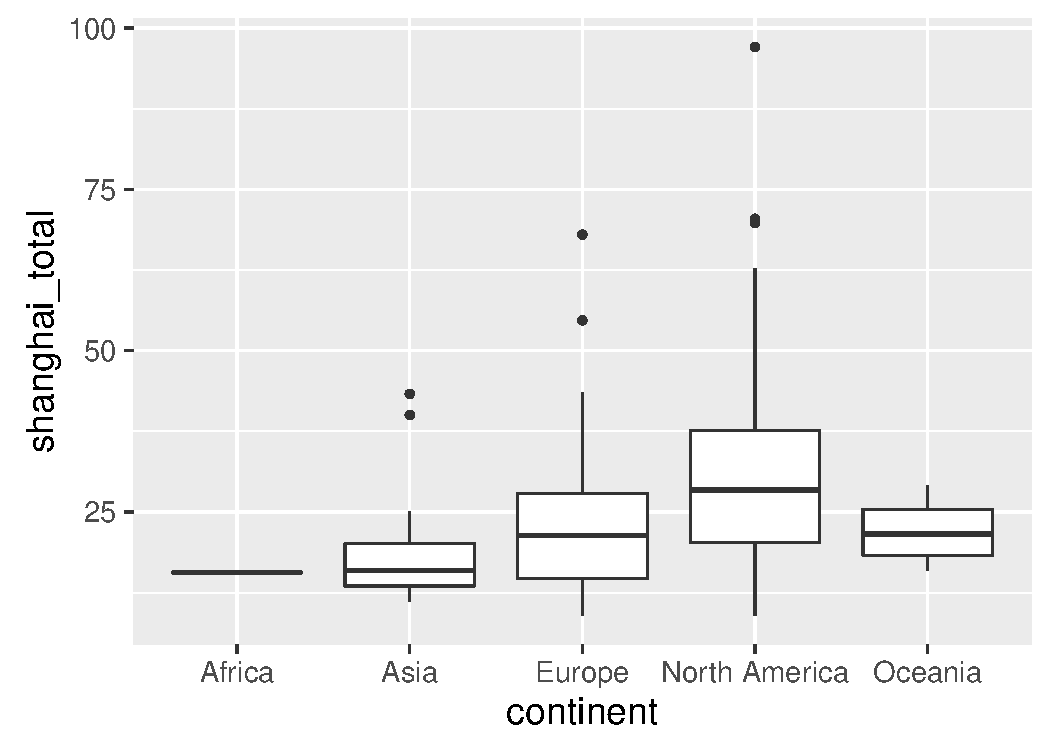
\includegraphics[width=0.5\textwidth]{graphs/continents_boxplot}
	\caption{Boxplots of Shanghai score per continent}
	\label{fig:boxcontinent}
\end{figure}

\begin{figure}
	\centering
	\begin{subfigure}{0.5\textwidth}
		\centering
		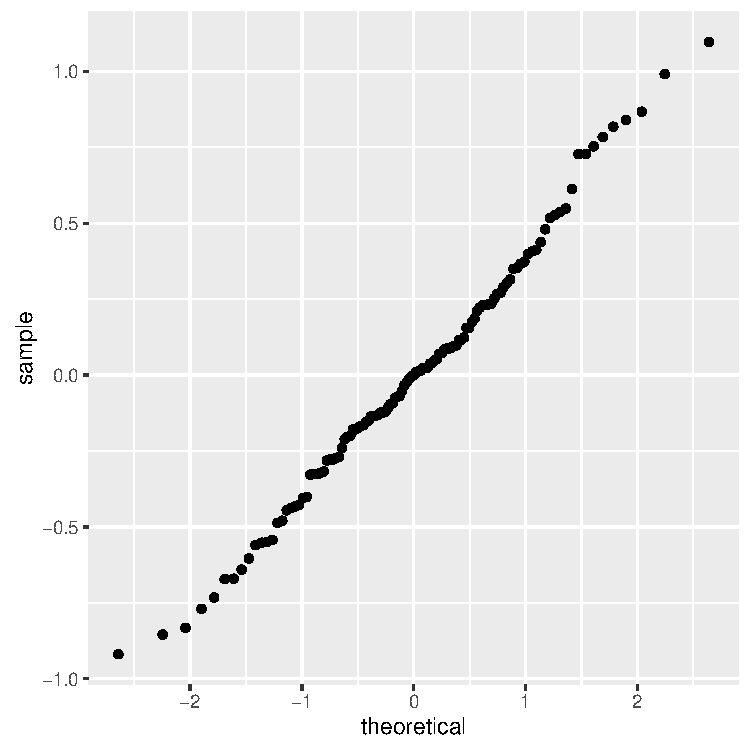
\includegraphics[width=\textwidth]{graphs/qq_final}
		\caption{QQ-plot of full model residuals.}
		\label{fig:qqfinal}
	\end{subfigure}%
	\begin{subfigure}{0.5\textwidth}
		\centering
		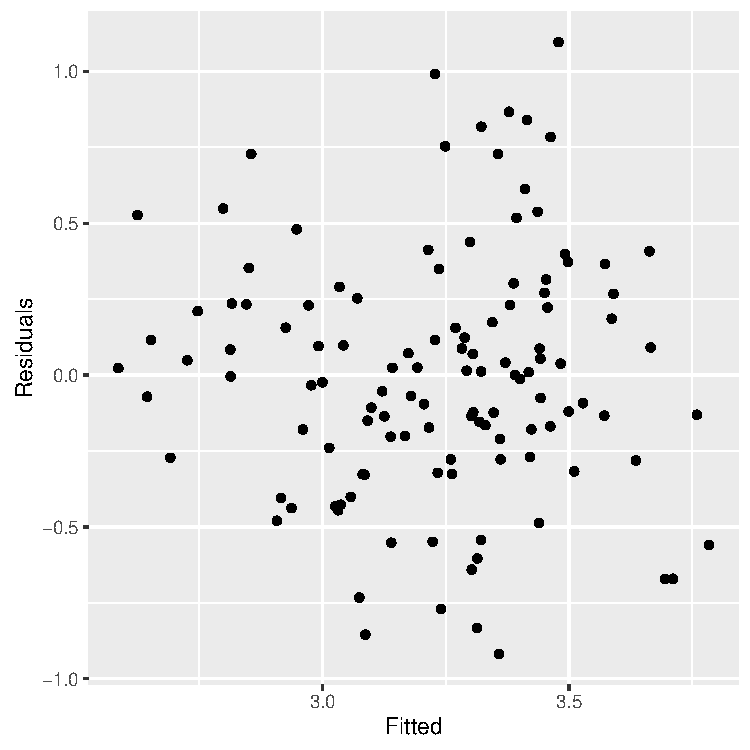
\includegraphics[width=\textwidth]{graphs/fit_res_final}
		\caption{Fitted against residuals of full model.}
		\label{fig:fitresfinal}
	\end{subfigure}
	\caption{Plots checking model assupmtions.}
\end{figure}

The dataset used in ANOVA and ANCOVA contains data
from universities 4 continents:
20 from Asia, 65 from Europe, 74 from North America and 8 from Oceania remain in
the dataset after removing entries with missing values. Statistics about the
dataset containing all variables can be found in Table~\ref{table:summary}. In
this table we see that some variables are likely not normal because their mean and median do not
overlap and the two quartiles are not equally far away from the median which
could be a problem for ANOVA, ANCOVA and linear regression.
Examples are the Shanghai score and the government expenditure per student.

As a first investigation into the dataset we plotted the histograms for all
variables in Figure~\ref{fig:hist} in Appendix~\ref{app: A}. The distribution for
most variables is not fully clear, but it can be assumed normal for the variables originating from the
Times dataset. The World Databank variables are too sparse to assume a
distribution for. The score response variable is clearly not normal, but most
likely exponentially distributed.

Figure~\ref{fig:boxcontinent} shows box plots of the Shanghai score per
continent using the dataset containing only Shanghai score and continent
variables.
In this figure North America appears to have the highest scores, followed by Europe and Oceania, but they are relatively close together. ANOVA
can be used to detect if the scores are significantly different. 

\subsection*{Assumptions}
To verify that the built final linear model is valid, its assumptions need to be
checked. The residuals
of the model are distributed normally, as illustrated in
Figure~\ref{fig:qqfinal}.
This was confirmed by a Shapiro test ($p=.5389$). To test for heteroscedasticity, the
fitted values were plotted against the residuals. Figure~\ref{fig:fitresfinal}
shows no particular shape, so we can assume the data is homoscedastic.

In addition to the normality and heteroscedacity assumptions, there should be no
interaction between the different continents in order to use ANCOVA.
Figure~\ref{fig:interaction} shows a fit for each variable and each continent.
Only for the student staff ratio variable the lines are reasonably parallel and
can no interaction be assumed.

In ANOVA, the group size is sufficiently large in all cases except Oceania,
which has size 8. This is a relatively small and should be taken into
consideration.

\subsection*{Hypothesis Testing}

% LM
\begin{table}
\centering
\begin{tabular}{lllll}
\hline
Coefficient & Estimate & Std. Error & t-value & $p$-value \\ 
\hline
(Intercept)                &  3.558e+00 & 2.588e-01 & 13.746 & $<$ 2e-16 *** \\
student:staff ratio        & -2.760e-02 & 8.154e-03 & -3.385 &0.000976 *** \\
international student ratio&  6.687e-01 & 2.376e-01 &  2.815 &0.005749 **  \\
expend per student       & -3.173e-02 & 1.111e-02 & -2.855& 0.005109 **  \\
number of students              &  1.319e-05 & 3.547e-06 &  3.720 &0.000311 *** \\
GPD                       &   1.112e-05 & 5.115e-06 &  2.175&0.031713 *   \\
interest rate                    & -7.342e-02 & 4.231e-02 & -1.735& 0.085392  \\
\hline		
\end{tabular}
\caption{Signif. codes: '***' $.001$, '**' $.01$, '*' $.05$.}
\label{table:lm}
\end{table}

The results of the multiple linear regression model are summarized in
Table~\ref{table:lm}. We found that the selected variables explained a
signficant part of the variance in university score in the Shanghai ranking,
$R^2 = .2563$, $F(6, 114) = 7.891$, $p = $ 4.035e-07. We find that increasing
the number of staff members per student has a very significant negative correlation
with the received score. The national education expenditure per student was also
found to have a negative correlation with the university score. We find that an
increasing number of students corresponds to an increase in the university score
as well as the ratio of international students to regular students, and the
national GDP per capita. The interest rate was not found to be significantly
related to the Shanghai university score.

% ANOVA
\begin{table}
\centering
\begin{tabular}{lllll}
\hline
Contrast & Diff.    & Lower 95\% & Upper 95\% &   $p$-value \\
\hline
Europe-Asia          &  0.17403870 &-0.12245257 &0.4705300 &0.4257300 \\
North America-Asia   &  0.46474087 & 0.17252272 &0.7569590 &0.0003369 \\
Oceania-Asia         &  0.19765325 &-0.28740417 &0.6827107 &0.7156506 \\
North America-Europe &  0.29070218 & 0.09359203 &0.4878123 &0.0010460 \\
Oceania-Europe        & 0.02361455 &-0.41082953 &0.4580586 &0.9989942 \\
Oceania-North America &-0.26708762 &-0.69862677 &0.1644515 &0.3778006 \\
\hline		
\end{tabular}
\caption{Results of a Tukey post hoc analysis.}
\label{table:tukey}
\end{table}        

% In the intercept-only model, all of the fitted values equal the mean of the
% response variable. Therefore, if the P value of the overall F-test is
% significant, your regression model predicts the response variable better than
% the mean of the response.
In the one-way ANOVA, we observed a significant main effect for continent on the
logarithm of the Shanghai score, $F(3, 163) = 8.1454$, $p =$ 4.365e-05. In
Table~\ref{table:tukey}, the results of a Tukey post hoc analysis are
summarized. We find that the mean logarithm of the Shanghai score are
significantly different between North-America and Europe, and between
North-American and Asia. In both cases, North-America has the higher score.

% Look how we did ancova in the assignment, did we miss anything?
In the ANCOVA, we found that there was a significant effect of the continent on
the logarithm of the Shanghai score, after controlling for the
student-to-staff member ratio, $F(3, 162)  = 7.2541 $, $p = .0001349$. The
covariate, the student-to-staff member ratio, was significantly related to the
logarithm of the Shanghai score, $F(1, 162)  = 6.9792  $, $p = .0090545 $.

\section*{Conclusion}
\label{Conclusion}
In this study we investigated what factors influence university quality.
More specifically, per-univerisity and per-country variables that were suspected
to influence ranking were collected by their relevance in literature and their
effect on the Shanghai university ranking was investigated. Three different models were built, one using ANOVA,
one using ANCOVA and one using multiple linear regression. Model assumptions
were validated before testing the hypotheses. Student-to-staff ratio,
international student ratio, government expenditure per student, university size
and GDP per capita were found to be significant while the interest rate on loans
was not. The continent a university is on was found to make a difference in
Shanghai score, even when controlling for student-to-staff ratio.

In our model we found that having more staff members per student has a positive
correlation with the Shanghai score. When there is more staff per student there is less
pressure on staff members and students have better access to staff, intuitively
increasing quality. 

While seemingly counterintuitive, we can explain the negative effect of
increased education spending per student on the quality of the best
universities. Countries that spend a lot per student often have strong public
universities, with regulations in place that limit the maximum tuition fee. This
tuition fee, combined with state funding per student, is the only source of
income for the university. Countries that do not invest as heavily into
education do not have these caps on the tuition fee, and as a result
universities in these countries can end up with a higher income per student than
in countries with more funding. With more money to spend per student the quality
of education and research can be improved, for example by allowing the
university to spend more on modern facilities that facilitate research and
learning.

The university size and international student ratio are also positively
correlated with the Shanghai score. This is in accordance with the literature,
which suggests that university size is an important factor, and also predicts a
link between flow of international students and Shanghai ranking. This is
probably an effect of universities that are perceived to have a high quality attracting more students, both from within a country and from abroad. University size could have an effect, as it is possible that larger universities are able to maintain more expensive resources.
For example, an H-NMR spectrometer costs millions, and many universities do
not own one. Owning one could improve the quality of education and research at this
university.

GDP per capita was found to correlate positively with the Shanghai score.
The GDP having a significant effect on Shanghai score can also be
explained in a straightforward manner since universities in a country with a
higher GDP are likely to be better equipped, both on staff and other aspects. 

In both ANCOVA and ANOVA we found that some continents have better scores than
others, ANOVA suggests that North America has the highest scores. North America
has significantly higher scores than Europe and Asia, but not significantly
higher than Oceania. This might be the case because Oceania's sample size is
low. In ANCOVA we again find that the continent is significant
after controlling for student to staff member ratio.

\section*{Discussion}
\label{Discussion}

A main discussion point in this study is the operationalization of the dependent variable. Quality of education is an abstract concept that is not measurable in one definite, objective way. We chose the Shanghai score, as opposed to another score, for its relative objectivity and it being used in the literature. However, the weights given to each of their criteria, as well as their choice of criteria, is subjective.

Another criticism is that we only look at the best universities, and not at an overall distribution of the quality of universities throughout the nation. This is a likely cause for the magnitude and direction of the effect of education spending, as a lower education spending per student likely benefits the few top universities, while disadvantaging most other institutions. For a better image we would consider all universities, but a dataset for such a study is much harder to come by.

A final problem is that not all countries are as strongly represented as others in the top 200 universities. Countries such as the United States of America and the Netherlands have a relatively strong presence in the top 200, whereas the entire continent of Africa is represented by one single entry, which had to be dropped in order to perform the ANOVA. Future studies would benefit from using a larger sample, in which various countries are represented in similar numbers.

Furthermore, a variable that might have been interesting but of which data was
not available is the student ratio of a country's population. This variable
is expected to be of interest because a larger student population could be an
impulse to improve univeristy quality.

\newpage

\bibliographystyle{apacite}
\bibliography{MyReferences}

\newpage
\appendix

\section{Plots}
\label{app: A}

\begin{figure}[H]
	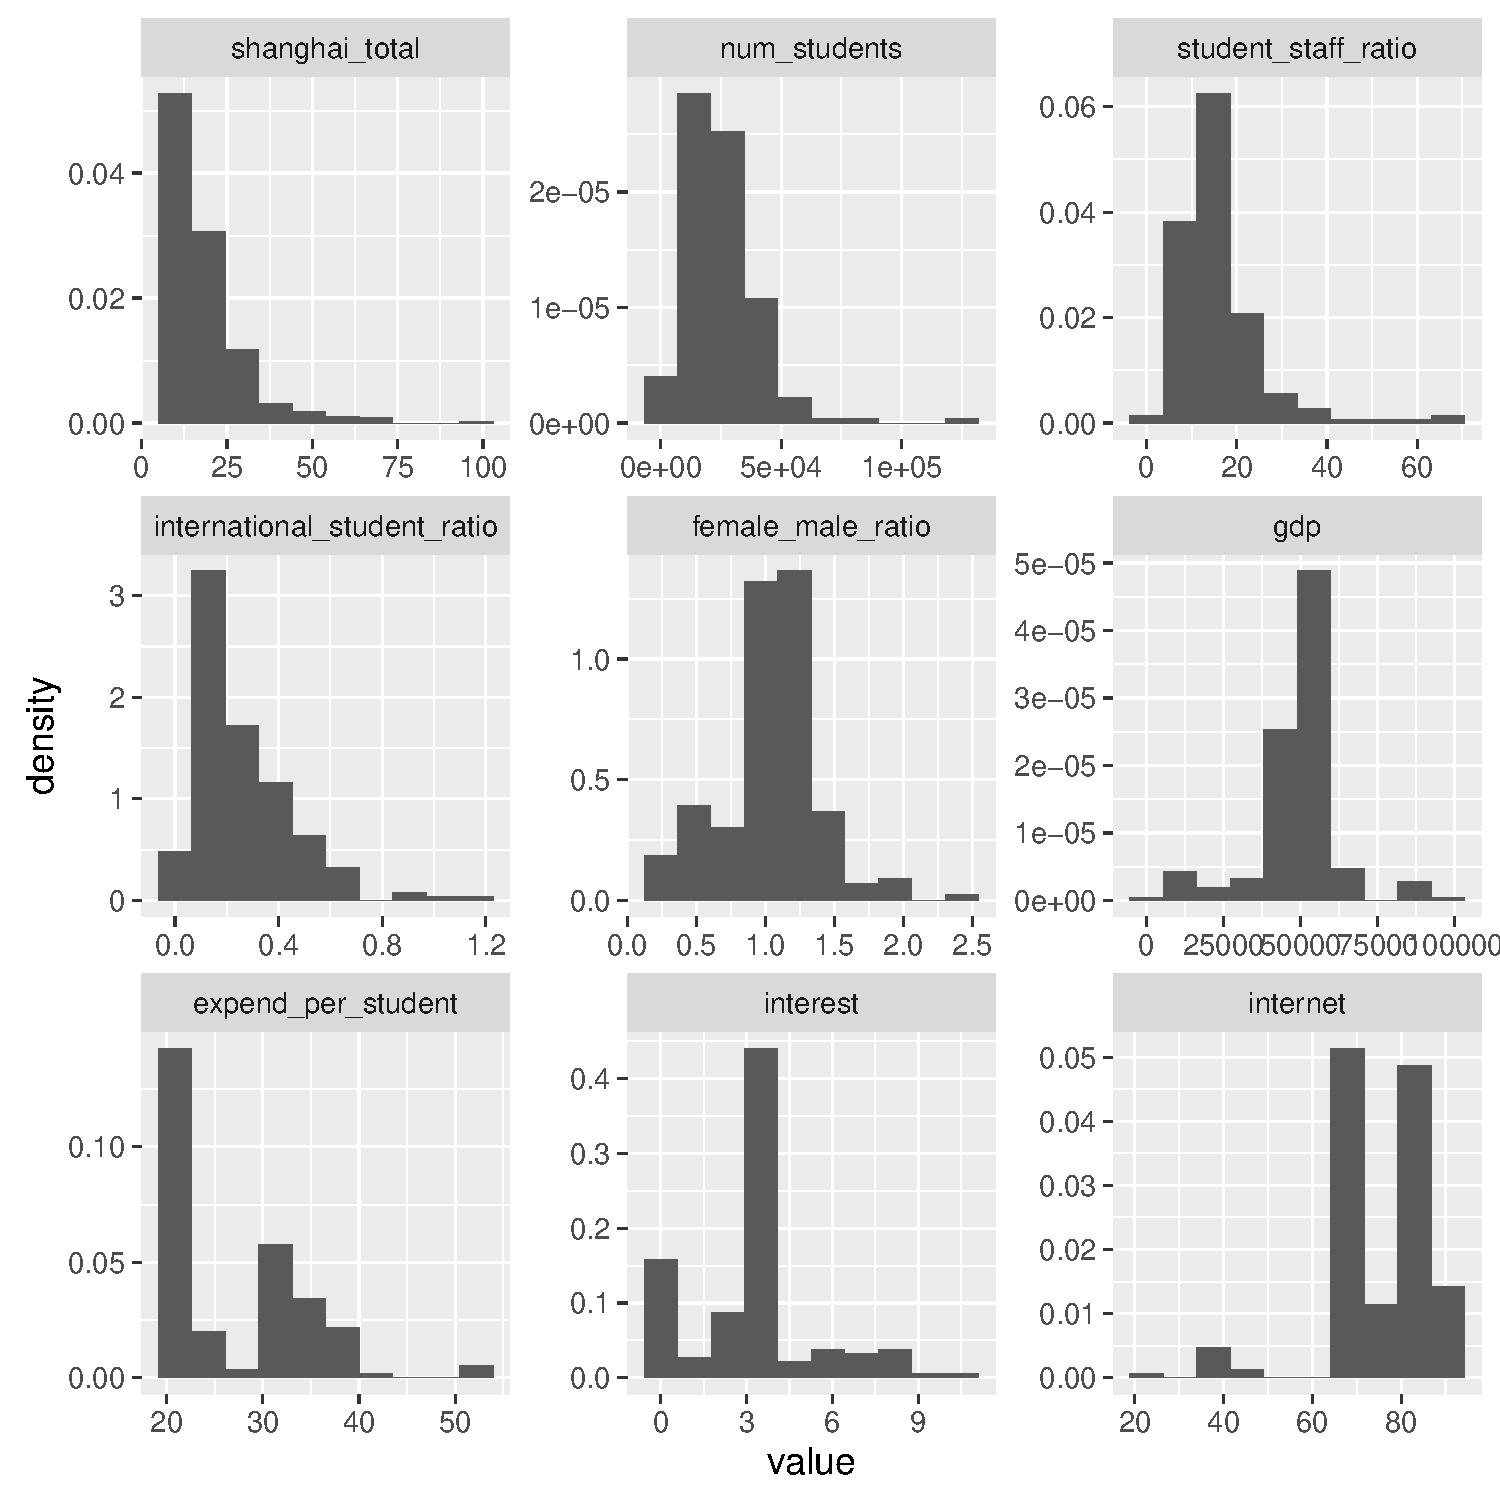
\includegraphics[width=\textwidth]{graphs/histograms}
	\caption{Histograms of the dataset.}
	\label{fig:hist}
\end{figure}

\begin{figure}[H]
	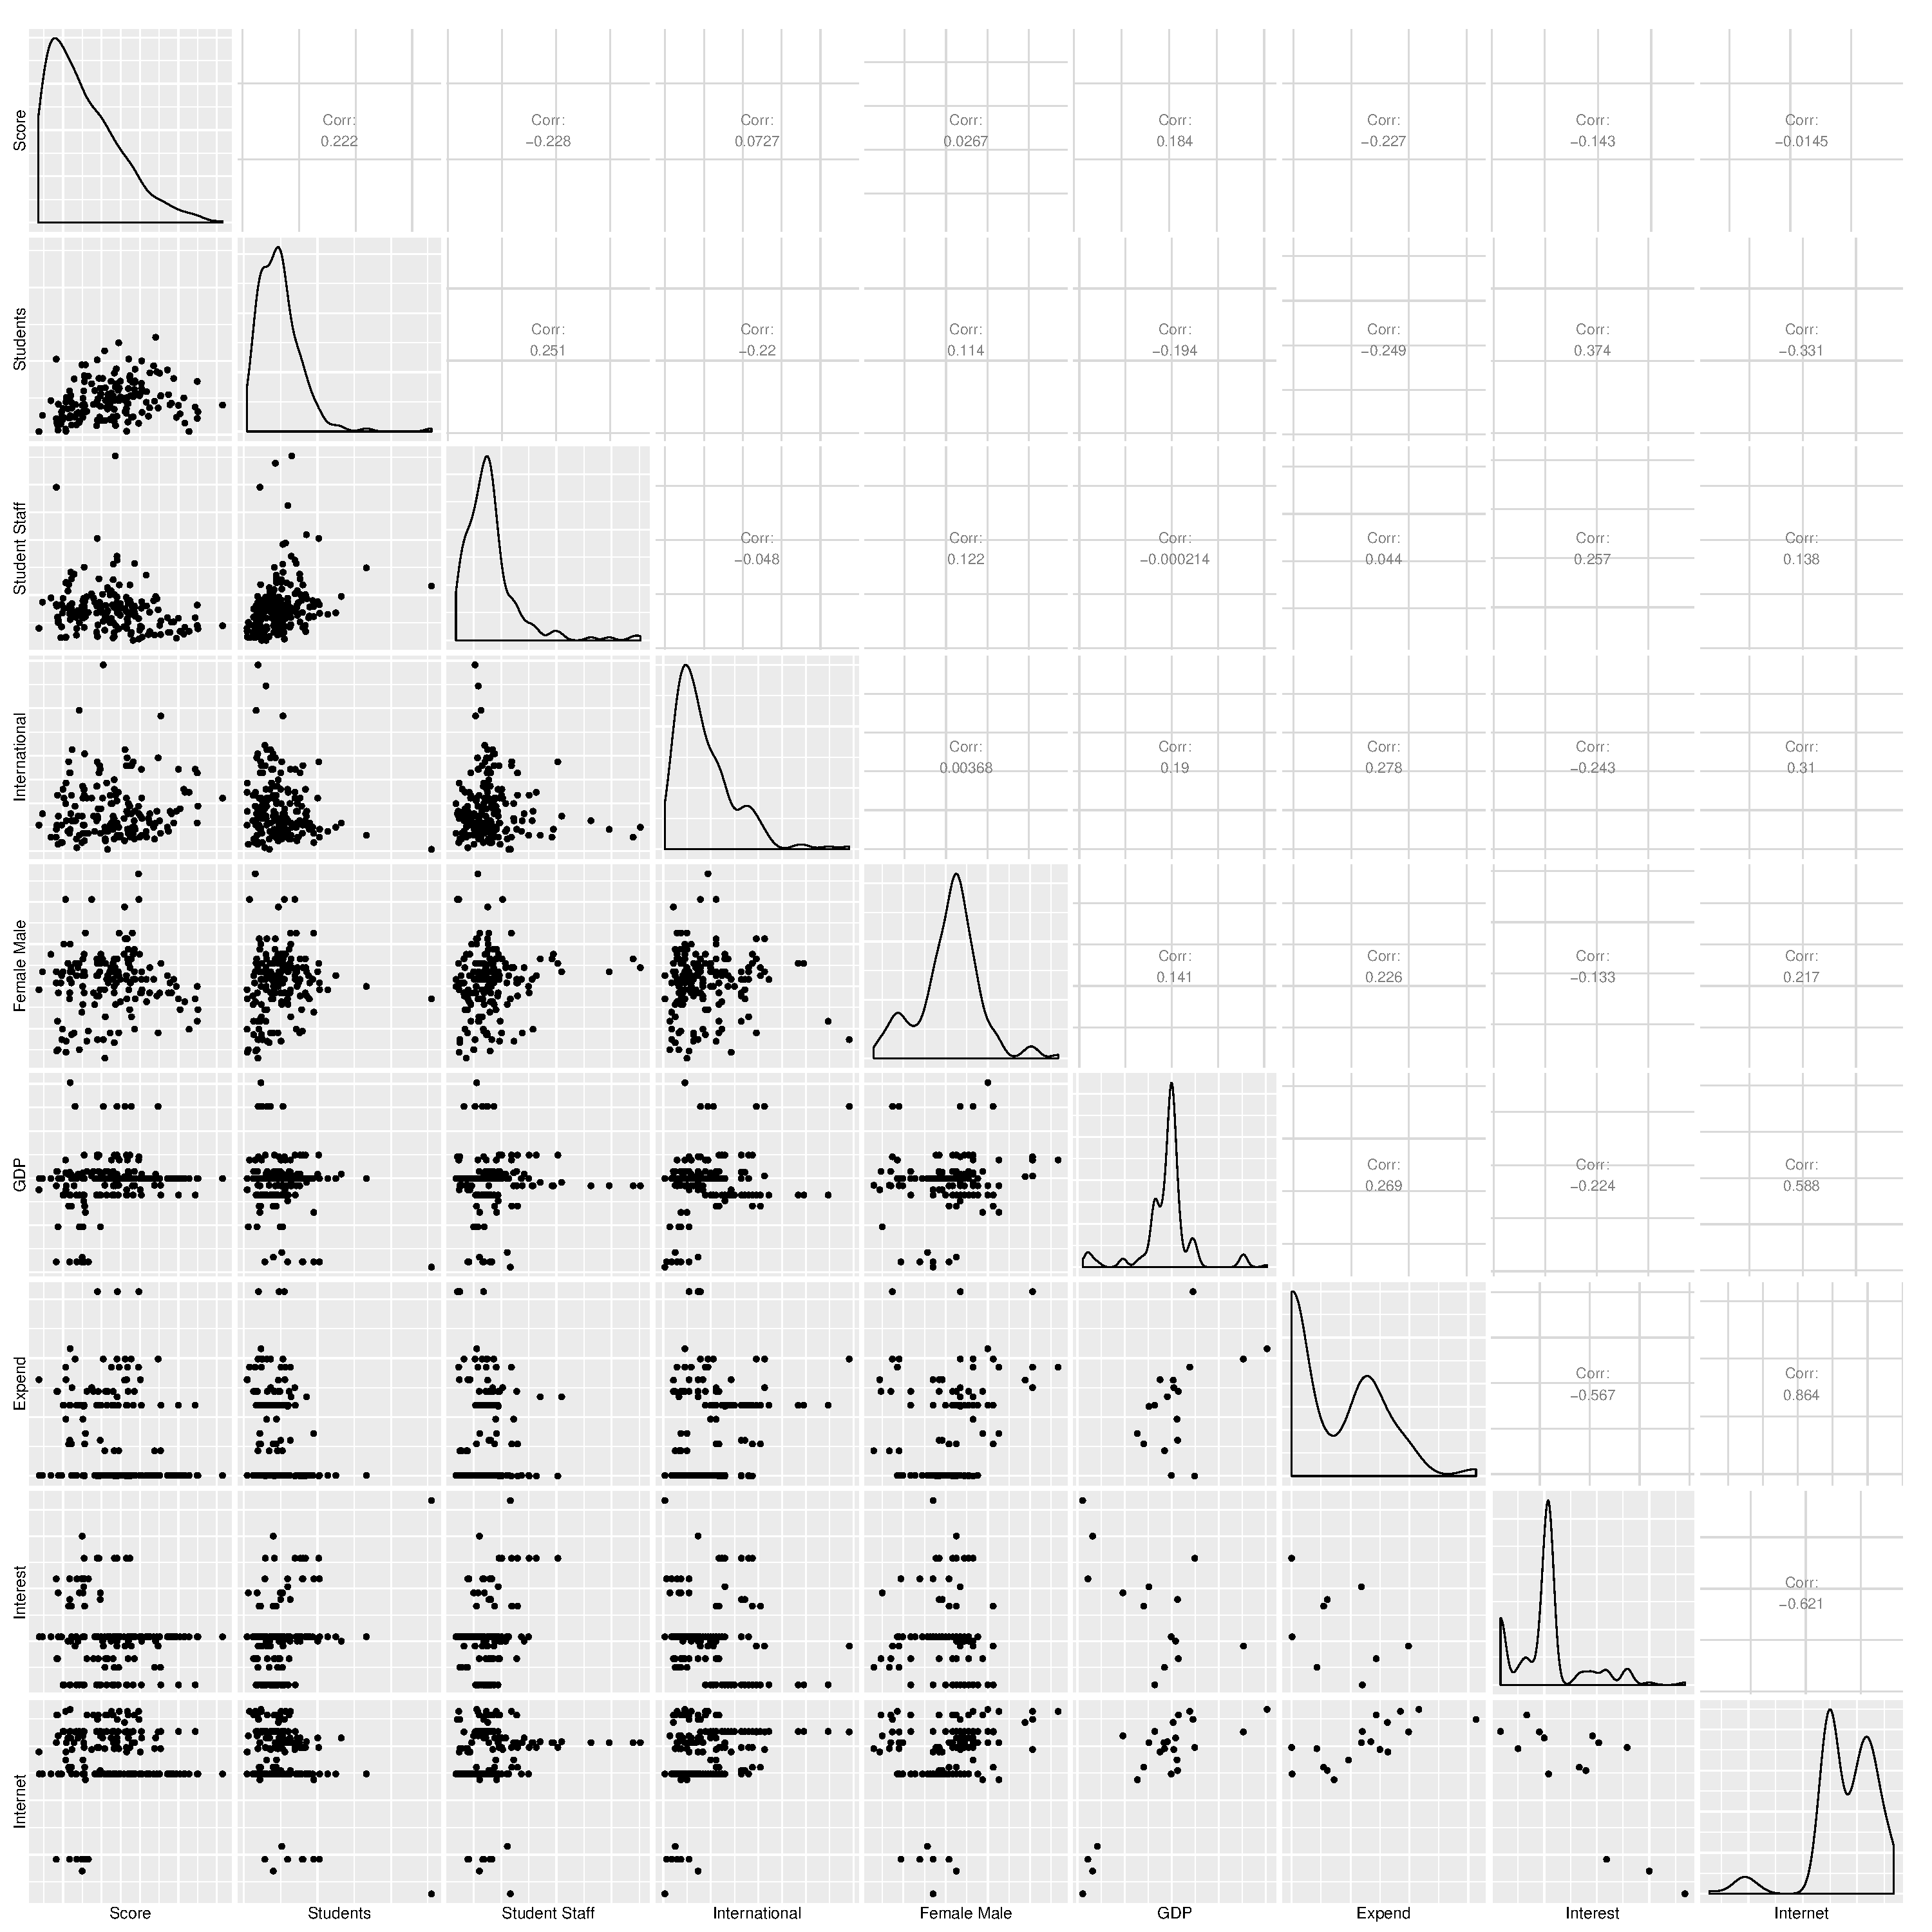
\includegraphics[width=\textwidth]{graphs/university-pairwise}
	\caption{Pairwise plots of the dataset with correlation.}
	\label{fig:pairwise}
\end{figure}

\begin{figure}[H]
	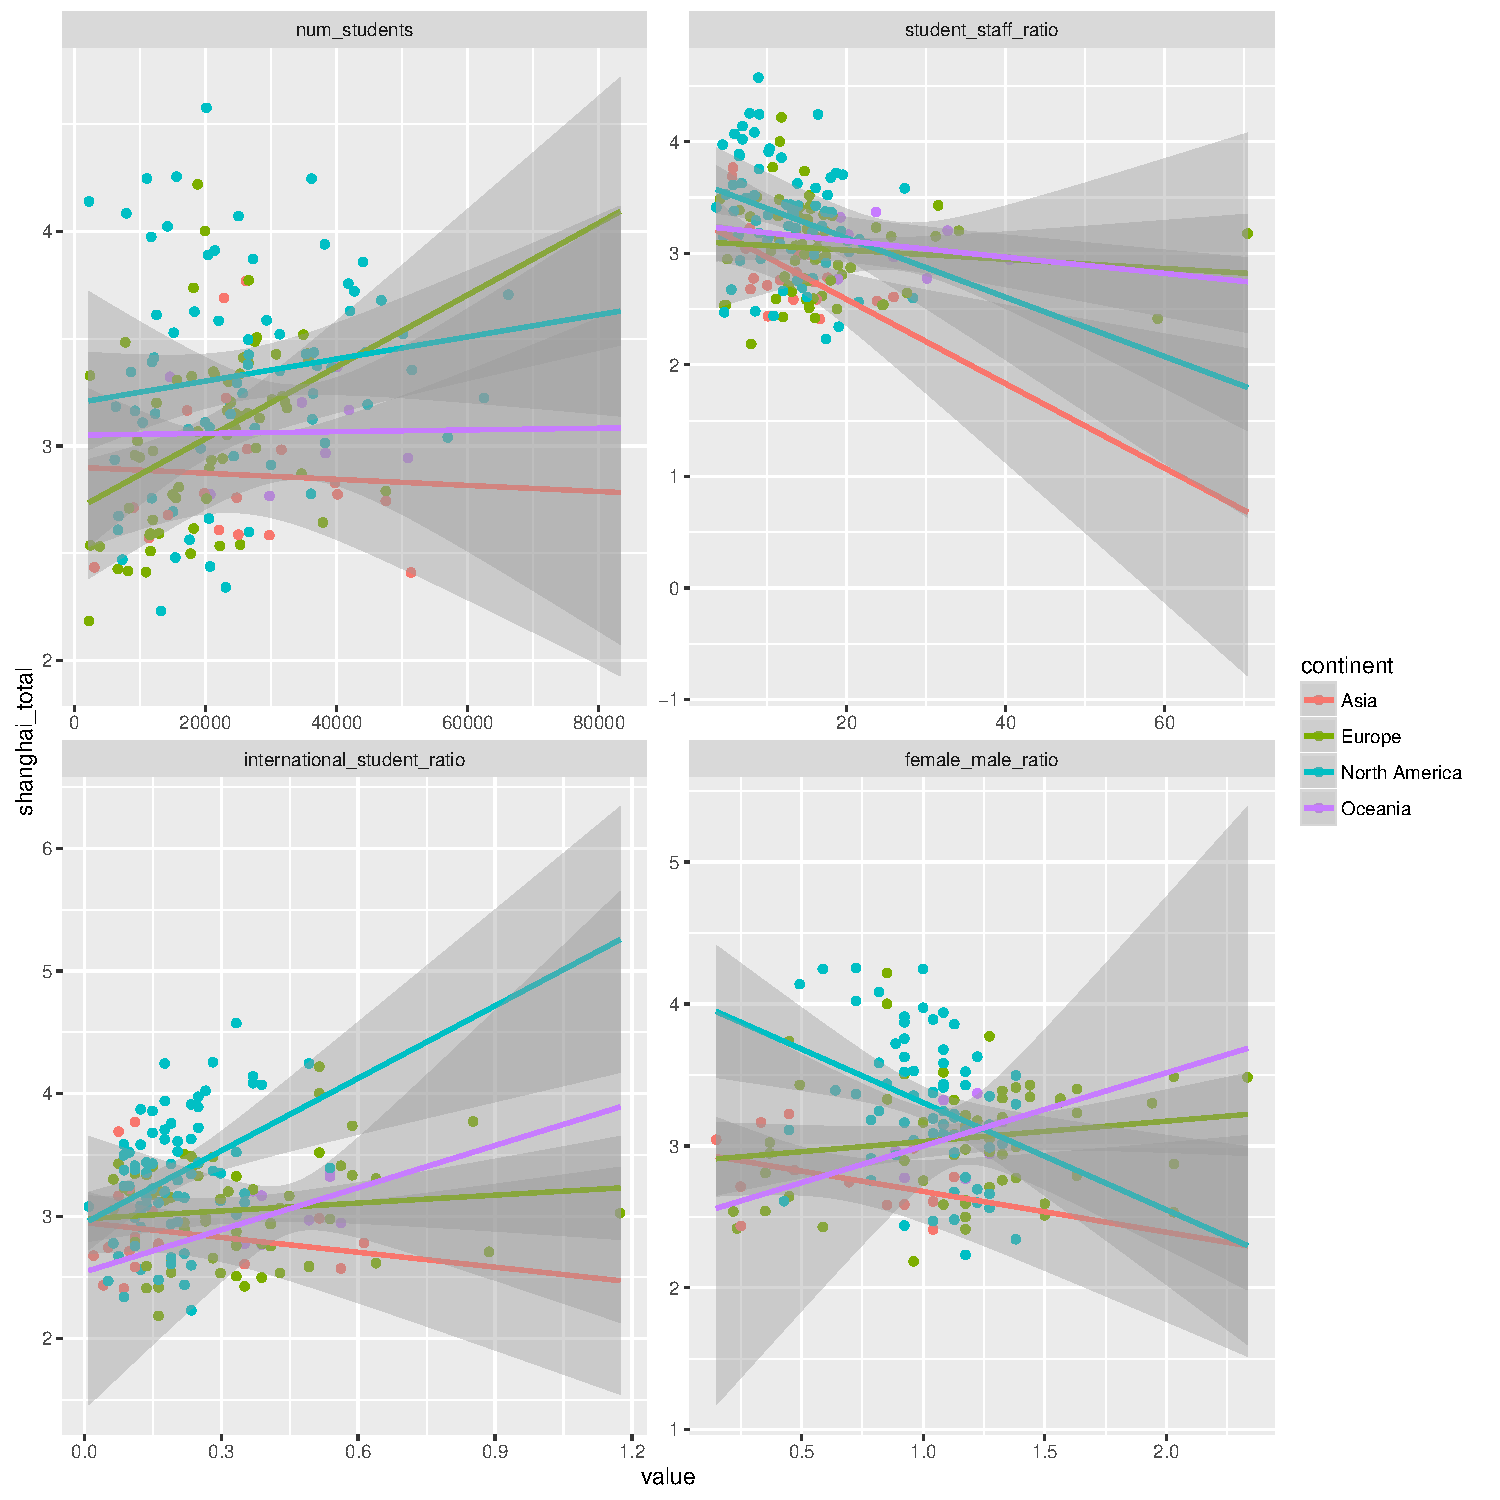
\includegraphics[width=\textwidth]{graphs/interaction_facets}
	\caption{Interaction between continents.}
	\label{fig:interaction}
\end{figure}

\end{document}